\section{集合间的基本关系}

本节要点:
\begin{itemize}
    \item 熟练掌握集合的各种关系。
\end{itemize}

~

集合的关系概念并没有什么难度。重点区分$a$和$\left\{ a \right\} $,前者是一个元素,后者是一个集合。

~

\begin{example}[综合运用4,难度:$\star $]
在平面直角坐标系中$C=\left\{ \left( x,y \right) \middle| y=x \right\} $表示直线$y=x$,从这个角度看,集合
\[
D=\left\{ \left( x,y \right) \middle| \left\{ \begin{array}{c}
	2x-y=1\\
	x+4y=5\\
\end{array} \right. \right\}
\]
表示什么?$C,D$间有什么关系?
\end{example}

解:

首先看$C$的表示方法$C=\left\{ \left( x,y \right) \middle| y=x \right\} $,各部分分析如下:
\begin{itemize}
    \item $C$:大写字母表示集合;
    \item $\left( x,y \right) $:一个有序实数对表示集合的元素是平面的点;
    \item $y=x$:一个等式表示$x,y$需满足的约束条件。
\end{itemize}
同理分析$D$的表示方法:
\begin{itemize}
    \item $D$:大写字母表示另一个集合;
    \item $\left( x,y \right) $:一个有序实数表示集合的元素依然是平面的点;
    \item $\left\{ \begin{array}{c}
        2x-y=1\\
        x+4y=5\\
    \end{array} \right. $:联立的两个等式表示$x,y$需要“同时”满足的两个约束条件。
\end{itemize}
不难发现,每个约束代表一条直线,若要“同时”满足两个约束条件,几何上表示两条直线的交点。
解方程组易得$x=y=1$,可见$C\supset D$。
$C,D$表示的几何图形如下:

\begin{figure}[h]
\centering
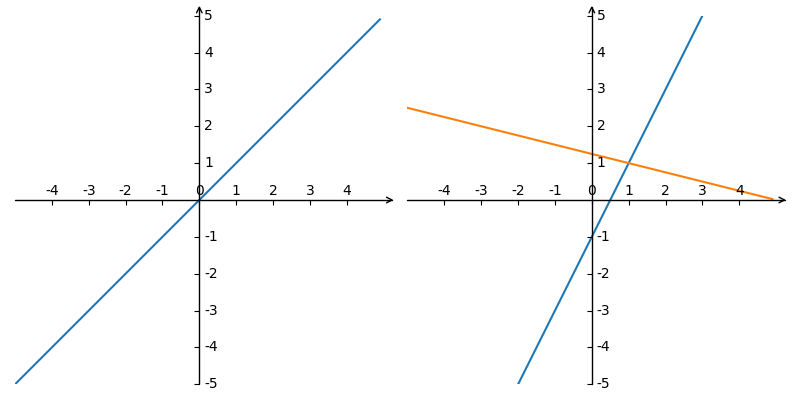
\includegraphics[height=4cm]{1.2-1.png}
\end{figure}

\begin{tcolorbox}
本题考察集合的概念和集合的描述方法。
\end{tcolorbox}




